\vspace{-0.1cm}
L’étude de l’existant permet d’identifier les points forts et les limites de l’application actuelle, ainsi que d’analyser les solutions similaires, afin d’orienter le développement d’une nouvelle version mieux adaptée aux besoins des utilisateurs.
\subsection{État actuel de l'application existante}
    L’application \textbf{PENTRA} (Figure~\ref{fig:PENTRA-V1-1}) constitue une première version d’un outil automatisé de tests de pénétration, développée dans le cadre d’un projet de fin d’études réalisé l’année précédente au sein de la société \textbf{ADDINN}. Elle a permis de poser les bases sur lesquelles s’appuient les évolutions futures envisagées dans le cadre de notre projet actuel.    
    \begin{figure}[H]
        \centering
        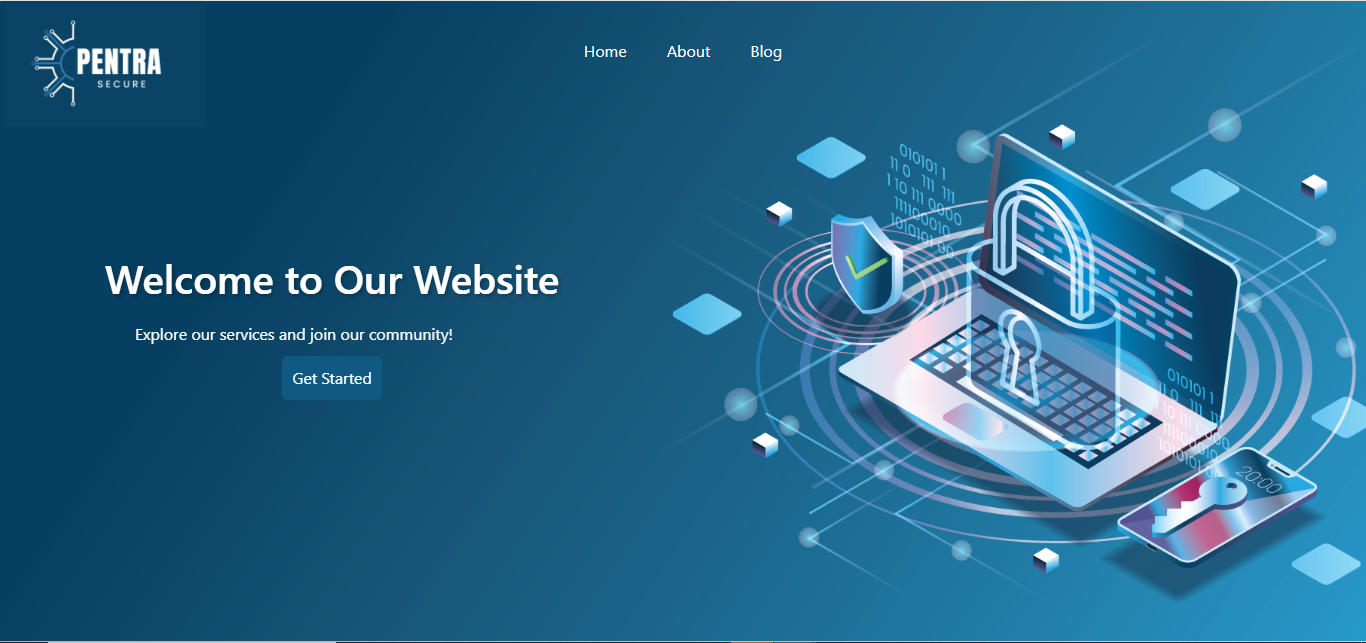
\includegraphics[width=\linewidth]{Annexe/PENTRA-V1/1.PNG}
        \caption{\centering Interface de la page d'accueil PENTRA}
        \label{fig:PENTRA-V1-1}
    \end{figure}
    \vspace{-0.3cm}
    \subsubsection{Analyse de la solution existante}  
        Il s’agit d’une solution de détection des vulnérabilités web, reposant principalement sur l’intégration de deux outils de scan réputés, largement reconnus dans le domaine de la cybersécurité :
        \begin{itemize}[label=$-$]
            \item  \textbf{OWASP ZAP (Zed Attack Proxy)}: Un scanner open source développé par l’OWASP pour identifier les failles de sécurité dans les applications web, telles que les injections SQL, les failles XSS, les problèmes d’authentification ou les erreurs de configuration. Il propose des analyses actives et passives, une interface graphique riche, ainsi qu’une API permettant son automatisation.\cite{zap}.
            \item \textbf{Wapiti}: un outil open source d’analyse de vulnérabilités web basé sur des tests d’injection, qui scanne les sites web à la recherche de failles comme les injections de commande, les XSS ou encore les inclusions de fichiers. Il se distingue par sa légèreté et son approche modulaire.\cite{wapiti}.  
        \end{itemize}
         Cette solution est développée avec Angular (version 15), FastAPI et PostgreSQL, et intègre les fonctionnalités clés suivantes:
        \begin{itemize}[label=$\bullet$, left=0.2cm]
             \item \textbf{Gestion de l’authentification\footnote{Voir annexe A: Figures \ref{fig:PENTRA-V1-2} et \ref{fig:PENTRA-V1-3}}:} Interfaces d'inscription et de connexion permettant aux utilisateurs de créer un compte et d'accéder à la plateforme via leurs identifiants.
            \item \textbf{Lancement du scan\footnote{Voir Annexe A: Figure \ref{fig:PENTRA-V1-4}}:} L’utilisateur saisit l’URL du site web à analyser dans le champ prévu. Les 2 outils de scan sont lancés et fonctionnent en mode multithread, ce qui permet de traiter plusieurs requêtes simultanément et d’accélérer le processus.
            \item \textbf{Tableau des résultats du scan par outil\footnote{Voir annexe A: Figures \ref{fig:PENTRA-V1-7}, \ref{fig:PENTRA-V1-8} et \ref{fig:PENTRA-V1-9}}:} Deux interfaces présentant les résultats des scans sous forme de tableaux, avec la possibilité de télécharger les rapports détaillés au format PDF, offrant ainsi une vue d'ensemble des vulnérabilités détectées.
            \item \textbf{Paramétrage de l’envoi des rapports\footnote{Voir annexe A: Figure \ref{fig:PENTRA-V1-10}}:} permet de configurer l’envoi automatique des rapports vers Slack, Jira et par e-mail.
            \item \textbf{Tableaux de bord\footnote{Voir annexe A: Figures \ref{fig:PENTRA-V1-5} et \ref{fig:PENTRA-V1-6}}:} Chaque outil dispose de sa propre interface, affichant les résultats des scans, leur progression, ainsi que des charts graphiques statiques.
            \item \textbf{Gestion des profils\footnote{Voir annexe A: Figures \ref{fig:PENTRA-V1-11}}:} Permet aux utilisateurs de modifier leurs informations personnelles.
            \item \textbf{Gestion des utilisateurs et des rapports de scan\footnote{Voir annexe A: Figures \ref{fig:PENTRA-V1-12} et \ref{fig:PENTRA-V1-13}}:} L’administrateur peut gérer les comptes utilisateurs ainsi que consulter, organiser et superviser les rapports des scans.
        \end{itemize}
    \subsubsection{Limites et critiques de la solution existante}
    L’application présente plusieurs lacunes affectant son ergonomie, ses performances et ses fonctionnalités. Ces limitations doivent être corrigées pour améliorer son efficacité globale.
        \begin{itemize}[label=\textcolor{red}{\ding{56}}]
            \item \textbf{Problèmes liés aux processus de scan et à la génération des rapports:}\\
            Les processus actuels de scan et de génération de rapports présentent plusieurs lacunes qui nuisent à la clarté des résultats, à l’ergonomie des interfaces et à l’efficacité globale de l’analyse. Parmi les problèmes relevés, on peut citer :
                \begin{itemize}[label=$\bullet$, left=-0.05cm]
                    \item \textbf{Surcharge d’informations:} Les tableaux des résultats des scans et les rapports générés sont excessivement longs et contiennent souvent des informations inutiles.
                   \item \textbf{Affichage de résultats non optimisés et non pertinents :} La présence de vulnérabilités avec un compteur égal à zéro, ainsi que de champs excessivement détaillés ou peu utiles, nuit à la lisibilité et complique l’analyse des résultats. Ce manque d’optimisation rend l’interprétation des rapports plus difficile et chronophage.
                    \item \textbf{Incohérence dans la structure des tableaux:} Les colonnes varient entre les outils, compliquant la comparaison des résultats. De plus, l'absence de filtres ou d'options de recherche pour trier les données rend leur exploitation moins efficace.
                    \item \textbf{Problèmes de progression des scans:} Les outils affichent la progression différemment: ZAP utilise une barre de progression, tandis que Wapiti le fait sous forme textuelle indiquant les modèles scannés, ce qui crée une incohérence.
                    \item \textbf{Navigation peu intuitive entre les interfaces des résultats:} La navigation entre les interfaces est confuse, ce qui complique la lecture et l’interprétation des résultats, notamment sur les tableaux de bord de Wapiti et ZAP ainsi que sur les deux tableaux de résultats, rendant l’analyse des vulnérabilités plus difficile.
                    \item \textbf{Mauvaise gestion des scans simultanés:} Le système actuel ne gère pas correctement les lancements parallèles ou successifs de plusieurs scans par le même utilisateur ou par plusieurs utilisateurs. Cela provoque une surcharge du backend, des conflits d’accès aux ressources, voire un blocage partiel de l’application. De plus, certains outils sont déclenchés plusieurs fois en parallèle, entraînant des erreurs d’exécution et empêchant la génération des rapports.
                    \item \textbf{Diffusion des rapports limitée :} Les e-mails contenant les rapports\footnote{Voir annexe A: Figure \ref{fig:PENTRA-V1-email}} sont trop basiques manquent de clarté et de modernité. Par ailleurs, l’envoi des rapports via Slack et Jira ne fonctionne pas de manière fiable. L’absence d’options de téléchargement aux formats HTML, JSON et CSV limite l’exportation et rend difficile l’analyse approfondie des résultats ou leur intégration avec d’autres outils.
                \end{itemize}
            \item \textbf{Couverture incomplète des types d’audits:} Le système actuel se concentre principalement sur les audits de sécurité mais ne prend pas en charge l’ensemble des autres formes d’analyse essentielles. Il n’intègre ni les tests fonctionnels ni les audits SEO. Cette limitation réduit la portée globale des évaluations et empêche une vision complète de l’état et de la qualité du site web.
            \item \textbf{Limites de la structure de la base de données :}La base repose sur deux tables (\texttt{utilisateur} et \texttt{rapport})\footnote{Voir Annexe A : Figure \ref{fig:PENTRA-db-initial}}, dans lesquelles les rapports sont stockés au format binaire sans structuration interne. Cette approche entraîne un manque de granularité empêchant l’interrogation directe d’éléments clés comme les vulnérabilités. Elle limite les capacités de recherche, de filtrage et d’agrégation des données via des requêtes SQL standards. À mesure que le volume de rapports augmente, cette structure nuit à la scalabilité et à la performance de la base en ralentissant l’accès aux données en augmentant la consommation de ressources et en rendant l’exploitation des données particulièrement difficile.
            \item \textbf{Problèmes des tableaux de bord statiques:} Les graphiques ne sont pas fonctionnels et restent statiques, empêchant une visualisation dynamique et claire des vulnérabilités. 
            \item \textbf{Navigation confuse :} La coexistence d’une barre supérieure et d’une barre latérale de navigation mal structurées crée une expérience utilisateur désorientante, avec des liens incohérents, inutiles ou bloqués.
            \item \textbf{Ancienne version d’Angular:}  L’application utilise actuellement Angular version 15, qui est dépassée et n’est plus utilisée par la société. Une migration vers une version plus récente est nécessaire.
            \item \textbf{Affichage non responsive:} Les interfaces ne sont pas totalement responsives, limitant une utilisation fluide sur différents types d’écrans (tablettes, mobiles, etc.).
            \item \textbf{Accès non sécurisé aux interfaces sans authentification:} Bien que l’accès au backend soit protégé par authentification (erreur 403 en cas d’accès non autorisé), l’utilisateur peut accéder librement au frontend (dashboard, historique des scans, page de scan) sans authentification, ce qui crée une incohérence dans la gestion des droits d’accès.
            \item \textbf{Absence de gestion des mots de passe:} Il manque les pages dédiées à la réinitialisation ou à la récupération du mot de passe oublié, ce qui empêche les utilisateurs de récupérer l’accès à leur compte en cas d’oubli.
         \end{itemize}
    Des améliorations importantes sont indispensables afin d’optimiser l’ergonomie, les fonctionnalités et la sécurité de l’application, tout en offrant une meilleure expérience utilisateur.